\section*{3. LLaDA-8B}

\subsection*{Problem \& Approach}
I didn't find time to do a comparison of the 5 methods with LLaDA. I was only able to perform an analysis of different number of denoising steps $T \in \{8, 16, 32, 64\}$ for the model, with no of tokens at each step to be unmasked linearly decreasing with no of steps.

\begin{table}[h]
\centering
\begin{tabular}{l c c c c c}
\toprule
\textbf{Steps} & \textbf{Overall Acc.} & \textbf{Level 1} & \textbf{Level 2} & \textbf{Level 3} & \textbf{Format Fails} \\
\midrule
$T = 8$  & 44.7\%  & 34.0\%  & 84.0\%  & 16.0\%  & 28 \\
$T = 16$ & 57.3\%  & 64.0\%  & 82.0\%  & 26.0\%  & 20 \\
$T = 32$ & \textbf{80.0\%} & \textbf{100.0\%} & \textbf{96.0\%}  & \textbf{44.0\%}  & \textbf{0} \\
$T = 64$ & 77.3\% & 100.0\% & 92.0\%  & 40.0\%  & 0 \\
\bottomrule
\end{tabular}
\caption{LLaDA-8B accuracy across diffusion steps.}
\label{tab:llada_results}
\end{table}

% \begin{figure}[h]
%     \centering
%     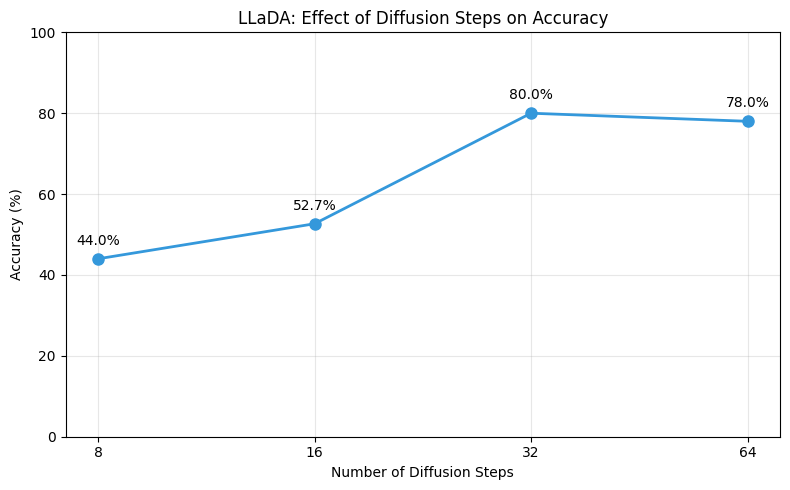
\includegraphics[width=0.48\textwidth]{llada_overall_acc_plot.png}
%     \hfill
%     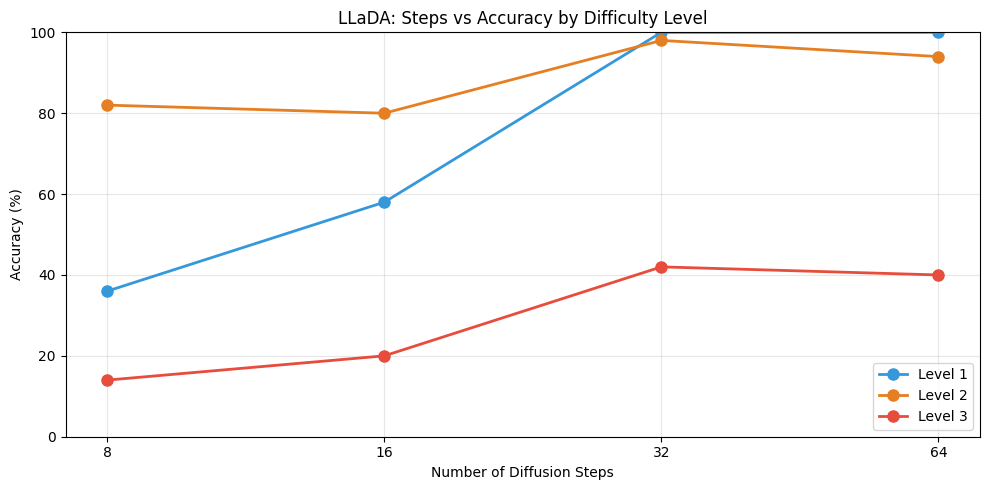
\includegraphics[width=0.48\textwidth]{llada_level_acc_plot.png}
%     \caption{Left: Overall accuracy vs. steps. Right: Level accuracy vs. steps.}
%     \label{fig:llada_plots}
% \end{figure}


Best performance observed at T = 32 (80\%). Format failures were relatively high at lower steps, likely because at each such step the model would need to unmask large number of tokens, including under-confident ones and stay with them. Therefore, it had less chances to correct its formatting. When I increased T to 64, its errors are not related to formatting but actual reasoning which could be a limitaiton with smaller T too but overshadowed by the formatting error.\\ \\

Example of such a T = 8 Failure: \\
\texttt{Problem: glorp(flarn(9, 7))} \\
\texttt{Expected: Final Answer: 16} \\
\texttt{Got: First, calculate flarn(9, 7) which is 9 + 7 = 16} \\

\vspace{0.5em}
Example of such a T = 64 Failure: \\
\texttt{Problem: glorp(flarn(snib(12, 4), 4))} \\ \texttt{Expected: Final Answer: 12} \\
\texttt{Got: Final Answer: 8} \\

Further analysis of the failure modes for each T could be done, and I shall do it when I find time.